\chapter{Dataset}\label{ch:Data}

This chapter examines the data set used in this project. It looks at how the data set is laid out to how the data was explored prior to preprocessing and training the model. 

\section{Dataset Origin}
The origin of the data set was previously discussed in the design chapter under the data set design section. The size of the data set is also mentioned in the chapter above.

\section{Data Exploration}
Learning the data set is an important stage to complete before training the model. It is useful as you can tell what the data set looks like to judge how much preprocessing takes place. some of the graphs and findings of the data exploration phase are examined below. The reason to explore data is to look for normality in the distributions of features, as well as looking for skewness and kurtosis.


The graph below shows a sample of the data set with the missing values being marked by a white cell and a valid sample as a black cell. the reason for it being only a sample of the data set is due to the size of the entire data set and the hardware available not being capable of running this missing data visualisation. This graph was produced using the missingno library.\\\\\\\\

\begin{figure}[h!]
  \centering
  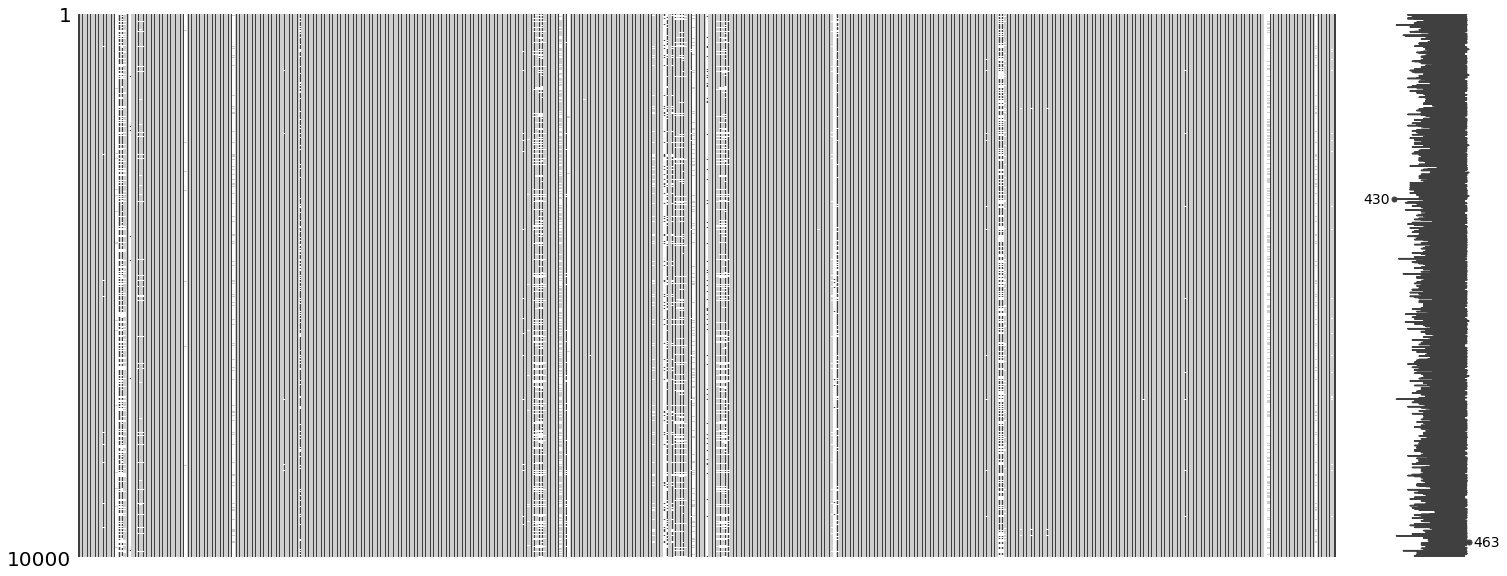
\includegraphics[width = (\textwidth)/2]{missingVals.png}
  \caption{Missingno matrix showing missing data for the first 10,000 samples}
  \label{fig:MV}
\end{figure}

As seen by the missing values matrix (figure \ref{fig:MV}) most of the features are either complete with only a few missing data or having non at all. The spark line on the side of the graph shows the completeness of the data on each row, with the maximum and the minimum marked out.Some of the features were then looked at to see the distribution of feature sets. The distribution for the furlongs of a race can be seen below.As you can see five furlongs seems to be the most common race length throughout the data set. 
\begin{figure}[h!]
  \centering
  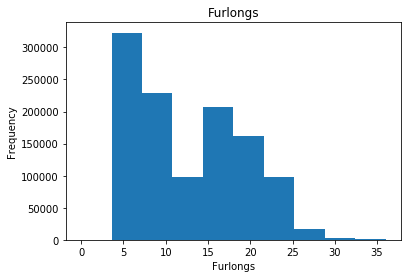
\includegraphics[width = (\textwidth)/2]{furlongs.png}
  \caption{furlongs distribution}
  \label{fig:fur}
\end{figure}

The horses age is another example of on of the features looked at below the distribution for the horses age for the whole data set can be seen along side a box blot showing the quartile ranges of the feature. As seen by figure \ref{fig:had} the most common age in the data set for horses is 4 years old, with the median being 5 as seen in figure \ref{fig:hab}. A further breakdown of the horses age by winner and non winner are discussed below.
\begin{figure}[H]
  \centering
  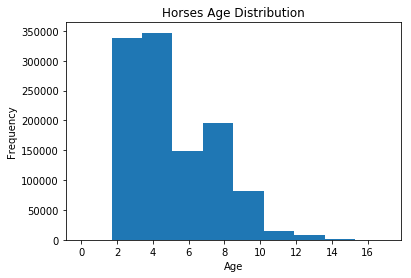
\includegraphics[width =(\textwidth)/2]{HorseAgeDistro.png}
  \caption{Horses age distribution}
  \label{fig:had}
\end{figure}
\begin{figure}[H]
  \centering
  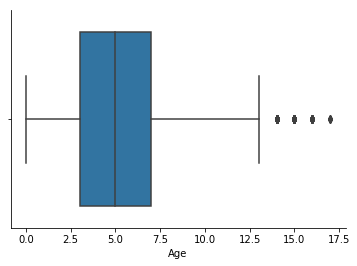
\includegraphics[width =(\textwidth)/2]{HorseAgeBoxplot.png}
  \caption{Horses age box plot}
  \label{fig:hab}
\end{figure}

As discussed further into this report, the model was changed to predict just a winner and non winner of the race. The visualisation of the distributions of the horses age for these labels can be seen below. As seen in figures \ref{fig:hawd} \& \ref{fig:hald} there is no underlying distribution to either category suggesting there is a level of randomness to the age of the winner horse, except for that most horses in this data set are 4 years old. 
\begin{figure}[H]
  \centering
  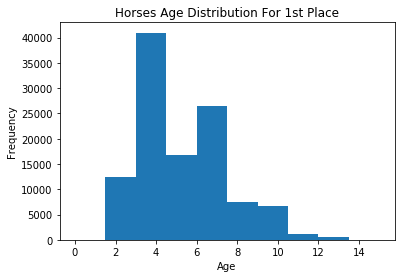
\includegraphics[width =(\textwidth)/2]{winnersAgeDistro.png}
  \caption{Horses age for 1st place distribution}
  \label{fig:hawd}
\end{figure}
\begin{figure}[H]
  \centering
  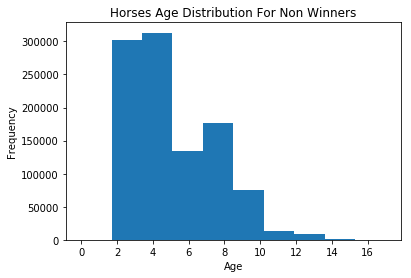
\includegraphics[width =(\textwidth)/2]{download.png}
  \caption{Horses age distribution for non winners}
  \label{fig:hald}
\end{figure}

\section{Conclusions}
The data within the data set is understood and the steps towards making the data set usable for training a neural network are clear and will take place during the preprocessing stage. Some of these steps will be talked about during the preprossessing section in the implementation chapter.

